\chapter{Luz y telescopios}
Desde tiempos antiguos, el ser humano ha sido curioso y se ha permitido alzar la mirada al cielo, observando así diferentes cuerpos astronómicos, tales como el Sol, la Luna, los planetas del sistema solar e incluso las estrellas de nuestra Galaxia. Estos objetos nos brindan información crucial a través de la luz que emiten o reflejan, permitiéndonos estudiarlos desde la Tierra.

Para explorar las regiones más lejanas del universo, ha sido indispensable la construcción de telescopios; instrumentos que amplifican nuestra capacidad de observar y analizar regiones del espacio extremadamente distantes de nuestro planeta. Sin embargo, para aprovechar al máximo las observaciones astronómicas que estos telescopios nos proporcionan, es fundamental desarrollar una comprensión profunda de los principios de la luz, como su naturaleza, comportamiento y cómo interactúa con la materia.

\section{Óptica de Telescopios}
\subsection{Naturaleza la luz}
En nuestra vida cotidiana, solemos referirnos a la luz como aquello que nuestros ojos pueden percibir. Sin embargo, gracias a la teoría del electromagnetismo y a las ecuaciones de Maxwell, entendemos que cuando partículas cargadas, como protones o electrones, se aceleran, generan ondas electromagnéticas. Estas ondas forman un vasto espectro conocido como el <<espectro electromagnético>>, del cual la luz <<óptica>> o <<visible>> constituye solo una pequeña porción. 

Las diferentes regiones del espectro electromagnético pueden ser descritas en términos de la longitud de onda, la frecuencia y la energía. La longitud de onda se mide en metros ($ m $) y se representa con el símbolo $ \lambda $ (letra griega lambda), mientras que la frecuencia se mide en unidades de hertz ($ \mathrm{1 Hz \equiv s^{-1}} $) y se representa con el símbolo $\nu$ (letra griega nu). Ambas cantidades se relacionan mediante:
\[ c = \lambda \nu, \]
donde $c$ es la velocidad de la luz en el espacio vacío y tiene un valor igual a $ 3\times 10^8 ~\mathrm{m ~ s^{-1}} $. La energía de la luz puede calcularse de manera simple con su frecuencia, gracias a la relación:
\[ E = h \nu, \]
donde $ h $ es la constante de Planck y tiene un valor numérico de $ 6.62607015\times 10^{-34} ~\mathrm{J~Hz^{-1}} $. Esta ecuación nos indica que a menor frecuencia (o de manera equivalente, a mayor longitud de onda), menor será la energía de la luz y viceversa.

La región óptica del espectro electromagnética está compuesta de luz cuya longitud de onda corresponde a todos los colores que percibimos, que van desde el azul ($ 420 \times 10^{-9} ~\mathrm{m} $) hasta el rojo ($ 640\times 10^{-9} ~\mathrm{m} $) y que pueden apreciarse en los arcoíris. En la Figura \ref{fig:em_spectrum} se muestra la región visible dentro de todo el espectro electromagnético.

\begin{figure}[htb]
  \centering
  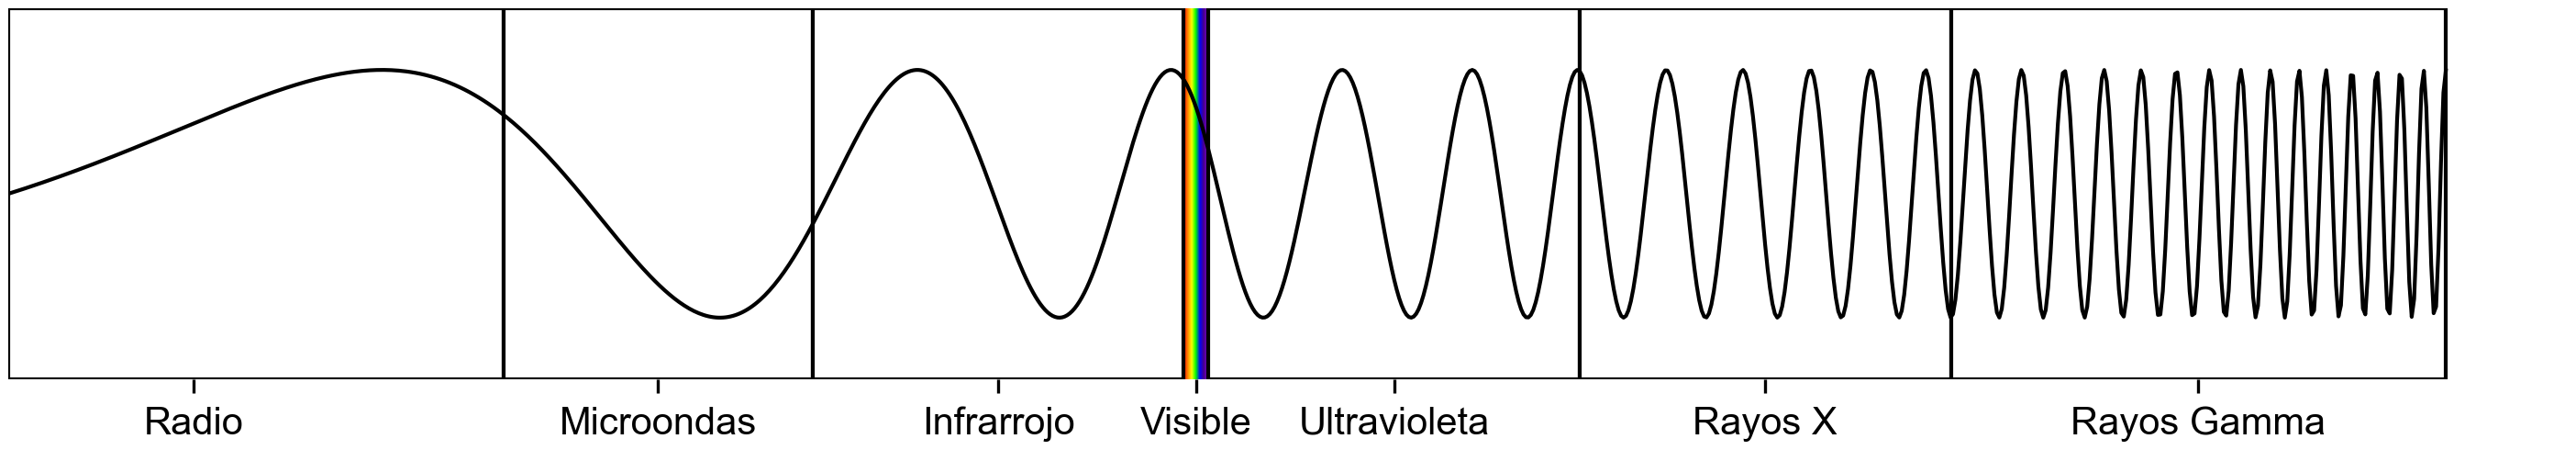
\includegraphics[width=\textwidth]{figures/em_spectrum.png}
  \caption{Espectro electromagnético}
  \label{fig:em_spectrum}
\end{figure}

Las diferentes porciones del espectro electromagnético reciben nombres específicos. Por ejemplo, la luz con longitudes de onda un poco más largas que el color rojo y que no somos capaces de ver se conoce como infrarrojo. Las ondas de radio son las ondas electromagnéticas con las longitudes de onda más largas y, por lo tanto, las menos energéticas. La región entre las ondas de radio y el infrarrojo se llama microondas, con longitudes de onda entre micrómetros y centímetros.

En el otro extremo del espectro, encontramos ondas electromagnéticas con longitudes de onda más cortas. Específicamente, la luz con longitud de onda más corta que el color violeta se llama ultravioleta. La luz con longitudes de onda aún menores se conoce como rayos X, y la luz con la longitud de onda más corta de todas se llama rayos gamma, que también es el tipo de radiación electromagnética más energética del universo.

\subsection{Principios básicos de óptica geométrica}
\subsubsection{Reflexión y refracción}
La óptica geométrica es una rama de la óptica que estudia y describe la luz en términos de rayos, donde un rayo se define como una línea imaginaria que indica la dirección en la que se propaga la luz. Esta dirección sigue un camino recto, permitiendo que la luz viaje entre dos puntos en el menor tiempo posible. Con esta aproximación de rayos, es posible describir la \textbf{refracción} y \textbf{reflexión} de la luz, los cuales son dos principios fundamentales que nos ayudarán a comprender cómo funcionan los telescopios. 

La refracción ocurre cuando la luz pasa a través de un material transparente, como el agua o el vidrio, mientras que la reflexión ocurre cuando la luz <<rebota>> sobre una superficie, como los espejos. Cuando la luz pasa de un material a otro (por ejemplo, del aire al agua), el camino que sigue la luz cambia de dirección, debido a que la velocidad de la luz es diferente en ambos medios. Para describir este cambio de dirección se utiliza la \textbf{Ley de Snell}:
\[ n_1 \sin\theta_1 = n_2 \sin \theta_2, \]
donde $ n_1 $ es el índice de refracción del primer material, $ n_2 $ es el índice de refracción del segundo material, $ \theta_1 $ es el ángulo incidente relativo a la normal de la superficie y $ \theta_2 $ es el ángulo de refracción relativo a la normal.

\begin{figure}[htb]
  \centering
  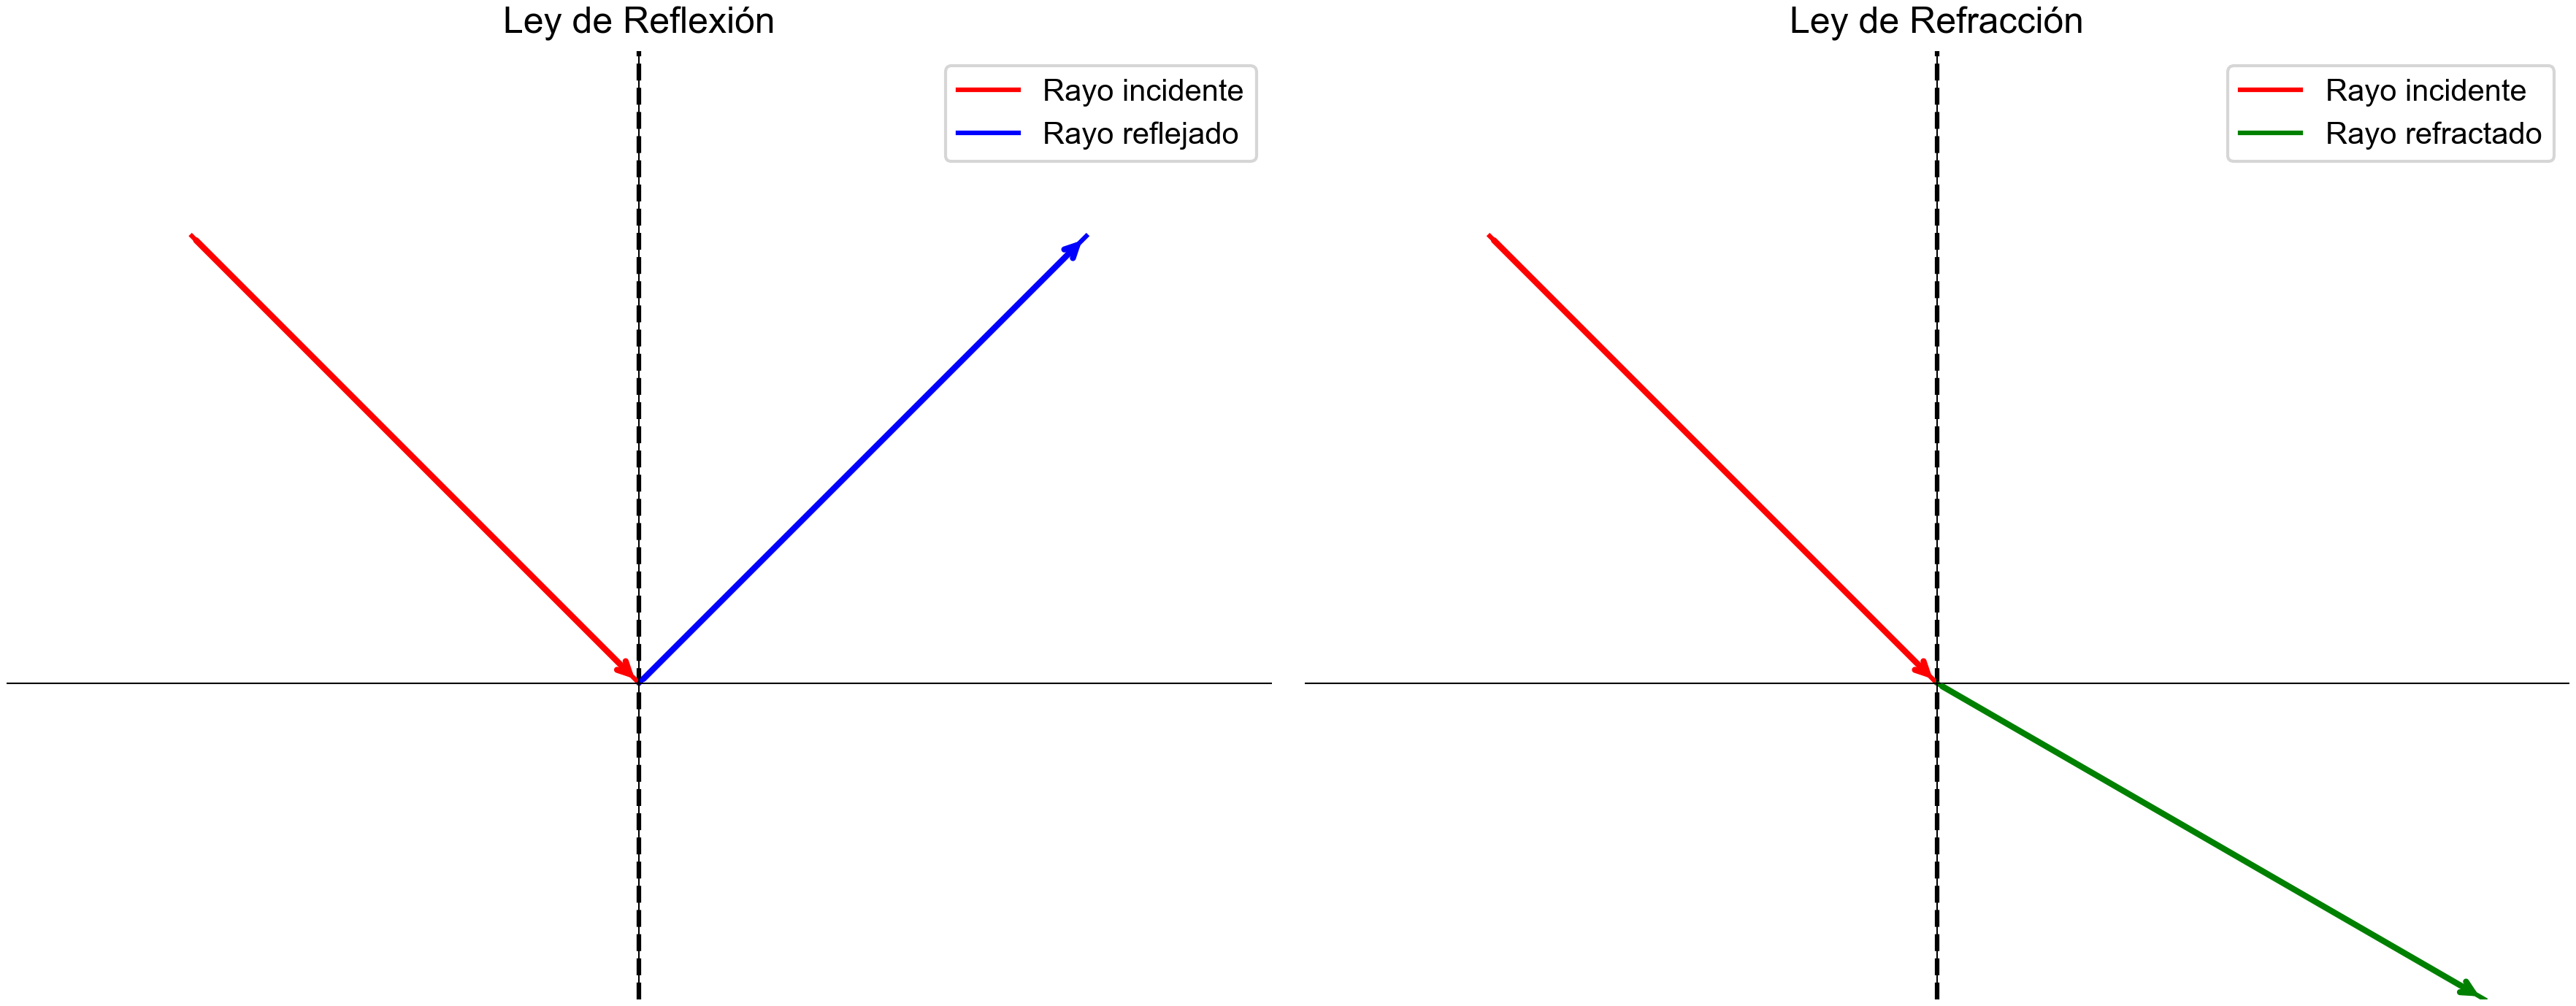
\includegraphics[width=\textwidth]{figures/light_laws.png}
  \caption{Leyes de refracción y reflexión. Figura adaptada de \citet{birney2006observational}.}
  \label{fig:light_laws}
  \end{figure} 

El índice de refracción de un material es simplemente el cociente entre la velocidad de la luz en el vacío y la velocidad de la luz en ese material: $ n = c/v $. Como ejemplo, el índice de refracción del vidrio es 1.520, el del diamante es 2.417 y el del agua es 1.333.

Para superficies reflectivas, ocurre un principio aún más simple: el ángulo de incidencia es igual al ángulo de reflexión, para todas las longitudes de onda de la luz. Esta es conocida como la \textbf{ley de reflexión}. La ley de refracción y ley de reflexión se ilustran en la Figura \ref{fig:light_laws}. Para más detalles sobre la propagación de la luz puedes consultar el libro <<Física Universitaria>> de \citet{young2020university} o <<Física>> de \citet{halliday2010physics}. 

\subsection{Telescopios}
Los telescopios están compuestos por un lente o espejo principal, el cuál es llamado el <<objetivo>> del telescopio. El objetivo del telescopio se encarga de recibir los rayos de luz provenientes de los objetos y desviarlos hacia el ocular, que es otro lente en el telescopio que se encarga de dirigir la luz hacia los ojos de las personas. Esta combinación de dos o más lentes/espejos es común en todos los telescopios y existen muchos diseños. El propósito es el mismo, producir una imagen magnificada o en el caso de fuentes puntuales, una imagen más brillante. En la Figura \ref{fig:galilean-refractor} se muestra el esquema de funcionamiento del telescopio refractor cuya invensión se le atribuye a Galileo Galilei y por lo tanto es conocido como el refractor Galileaon. 

\begin{figure}[htb]
  \centering
				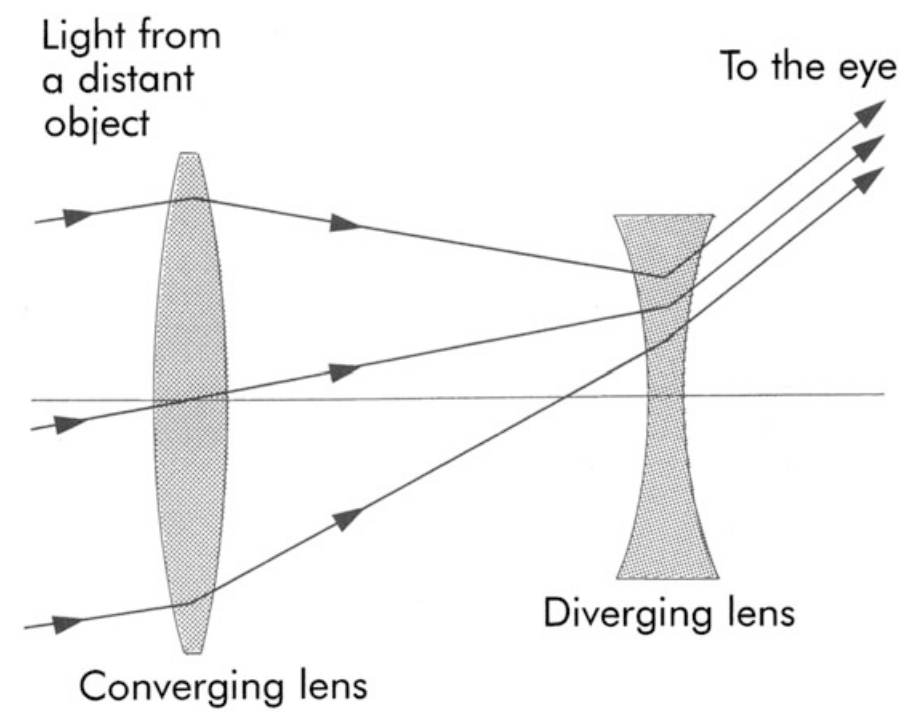
\includegraphics[width=0.7\textwidth]{figures/galilean-refractor.png}
				\caption{Óptica de un telescopio refractor Galileano. Figura tomada de \citet{kitchin2013telescopes}}
				\label{fig:galilean-refractor} 
\end{figure}

La estructura del refractor Galileano consiste de un lente convergente que orienta los rayos de luz hacia un lente divergente que luego envía la luz hacia los ojos. Si bien este tipo de telescopios funciona para aumentar el tamaño de las imágenes, sufre de algunos problemas, el más importante de mencionar es el de las <<aberraciones>> \citep{kitchin2013telescopes}. Las aberraciones consisten en que los rayos de luz de una fuente no convergen en un mismo punto cuando pasan a través de los lentes. 

En los telescopios de refracción ocurren dos tipos de aberraciones: la aberración esférica y la aberración cromática. La aberración esférica ocurre cuando objetos a diferentes distancias del eje óptico se concentran en focos a diferentes distancias y por lo tanto no existe un punto donde colocar el ocular para generar una imagen nítida. La aberración cromática es muy similar y ocurre cuando los rayos a diferentes longitudes de onda convergen en diferentes puntos. 

A diferencia de los lentes, los espejos no sufren del problema de la aberración cromática, ya que la reflexión es independiente de la longitud de onda. Si además se cambia la forma esférica por una parabólica, se elimina también el problema de la aberración esférica. Esto condujo a una preferencia hacia los telescopios de reflexión usando superficies parabólicas, que utilizan espejos primarios paraboloides y un espejo secundario elipsoide que luego envía los rayos de luz hacia el ocular. Dicha estructura se muestra en la Figura \ref{fig:paraboloidal-telescope} y es conocido como un telescopio Gregoriano.

\begin{figure}[htb]
  \centering
	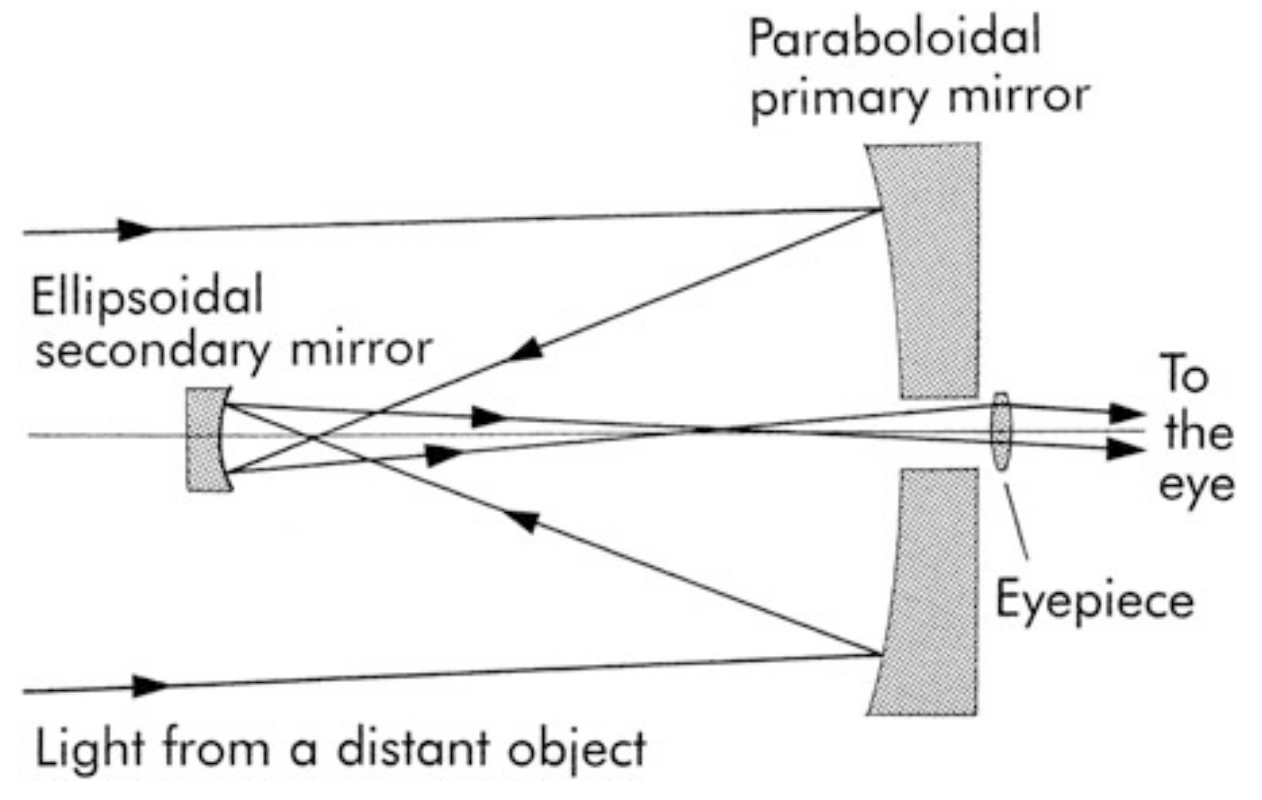
\includegraphics[width=0.8\textwidth]{figures/paraboloidal-telescope.png}
	\caption{Esquema de un telescopio Gregoriano. Figura tomada de \citet{kitchin2013telescopes}.}
	\label{fig:paraboloidal-telescope} 
\end{figure}

Una de las variaciones de los telescopios Gregorianos son los telescopios de Cassegrain, que reemplaza el espejo secundario elíptico por un espejo convexo hiperbólico. Diseños de los telescopios de Cassegrain o ligeras variaciones se siguen utilizando. Por ejemplo, tanto el Telescopio Espacial Hubble (HST) y el Keck de $ 10 \mathrm{~m} $ se basan en ese diseño. En la Figura \ref{fig:types-of-telescopes} se muestran los principales tipos de telescopios.

\begin{figure}[htb]
  \centering
				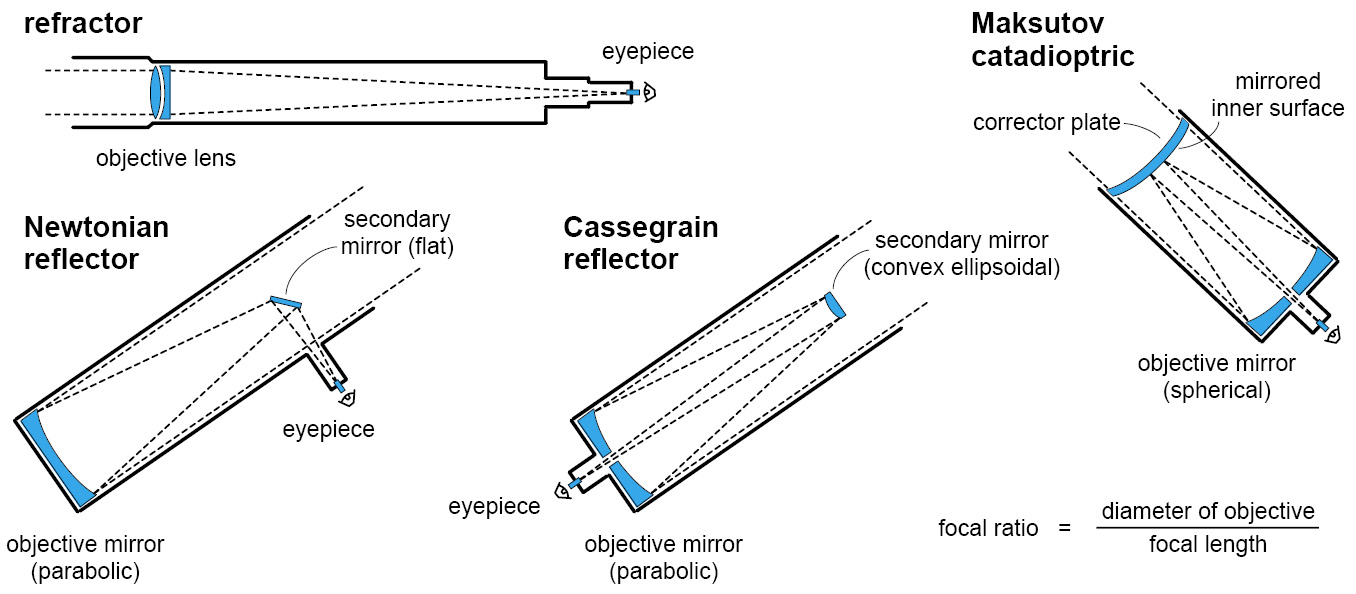
\includegraphics[width=\textwidth]{figures/types-of-telescopes.jpg}
				\caption{Algunos diseños de telescopios ópticos. Fuente: \href{https://assa.saao.ac.za/how-to-observe/equipment/telescopes/}{Astronomical Society of Southern Africa}.}
				\label{fig:types-of-telescopes} 
\end{figure}

\subsection{Observaciones a través de la atmósfera}
El ser humano y todas las formas de vida en la Tierra existen gracias a la atmósfera, que no permite el paso de la luz a ciertas longitudes de onda. Particularmente, toda la luz con longitud de onda más corta que el ultravioleta es absorbida por la atmósfera. De no ser así, la vida en la Tierra no sería posible. Todo esto es muy conveniente, pero representa un problema para los astrónomos, ya que no nos permite ver el espacio en todas las longitudes de onda desde la superficie de la Tierra. 

El panel superior de la Figura \ref{fig:atmosphere-atenuation} muestra los tamaños de las longitudes de onda en cada región del espectro electromagnético, desde los rayos gamma hasta las ondas de radio. El panel inferior muestra un gráfico que describe la transparencia de la atmósfera terrestre en cada región del espectro electromagnético. En esa figura, una transmisión del 100\% indicaría que la atmósfera es totalmente transparente y por lo tanto toda la luz logra llegar a la superficie terrestre. Como puedes ver, las partículas de oxígeno y nitrógeno en la atmósfera absorben a los rayos gamma y los rayos X en su totalidad, mientras que casi todos los rayos ultravioleta son absorbidos por el ozono. 

\begin{figure}
  \centering
	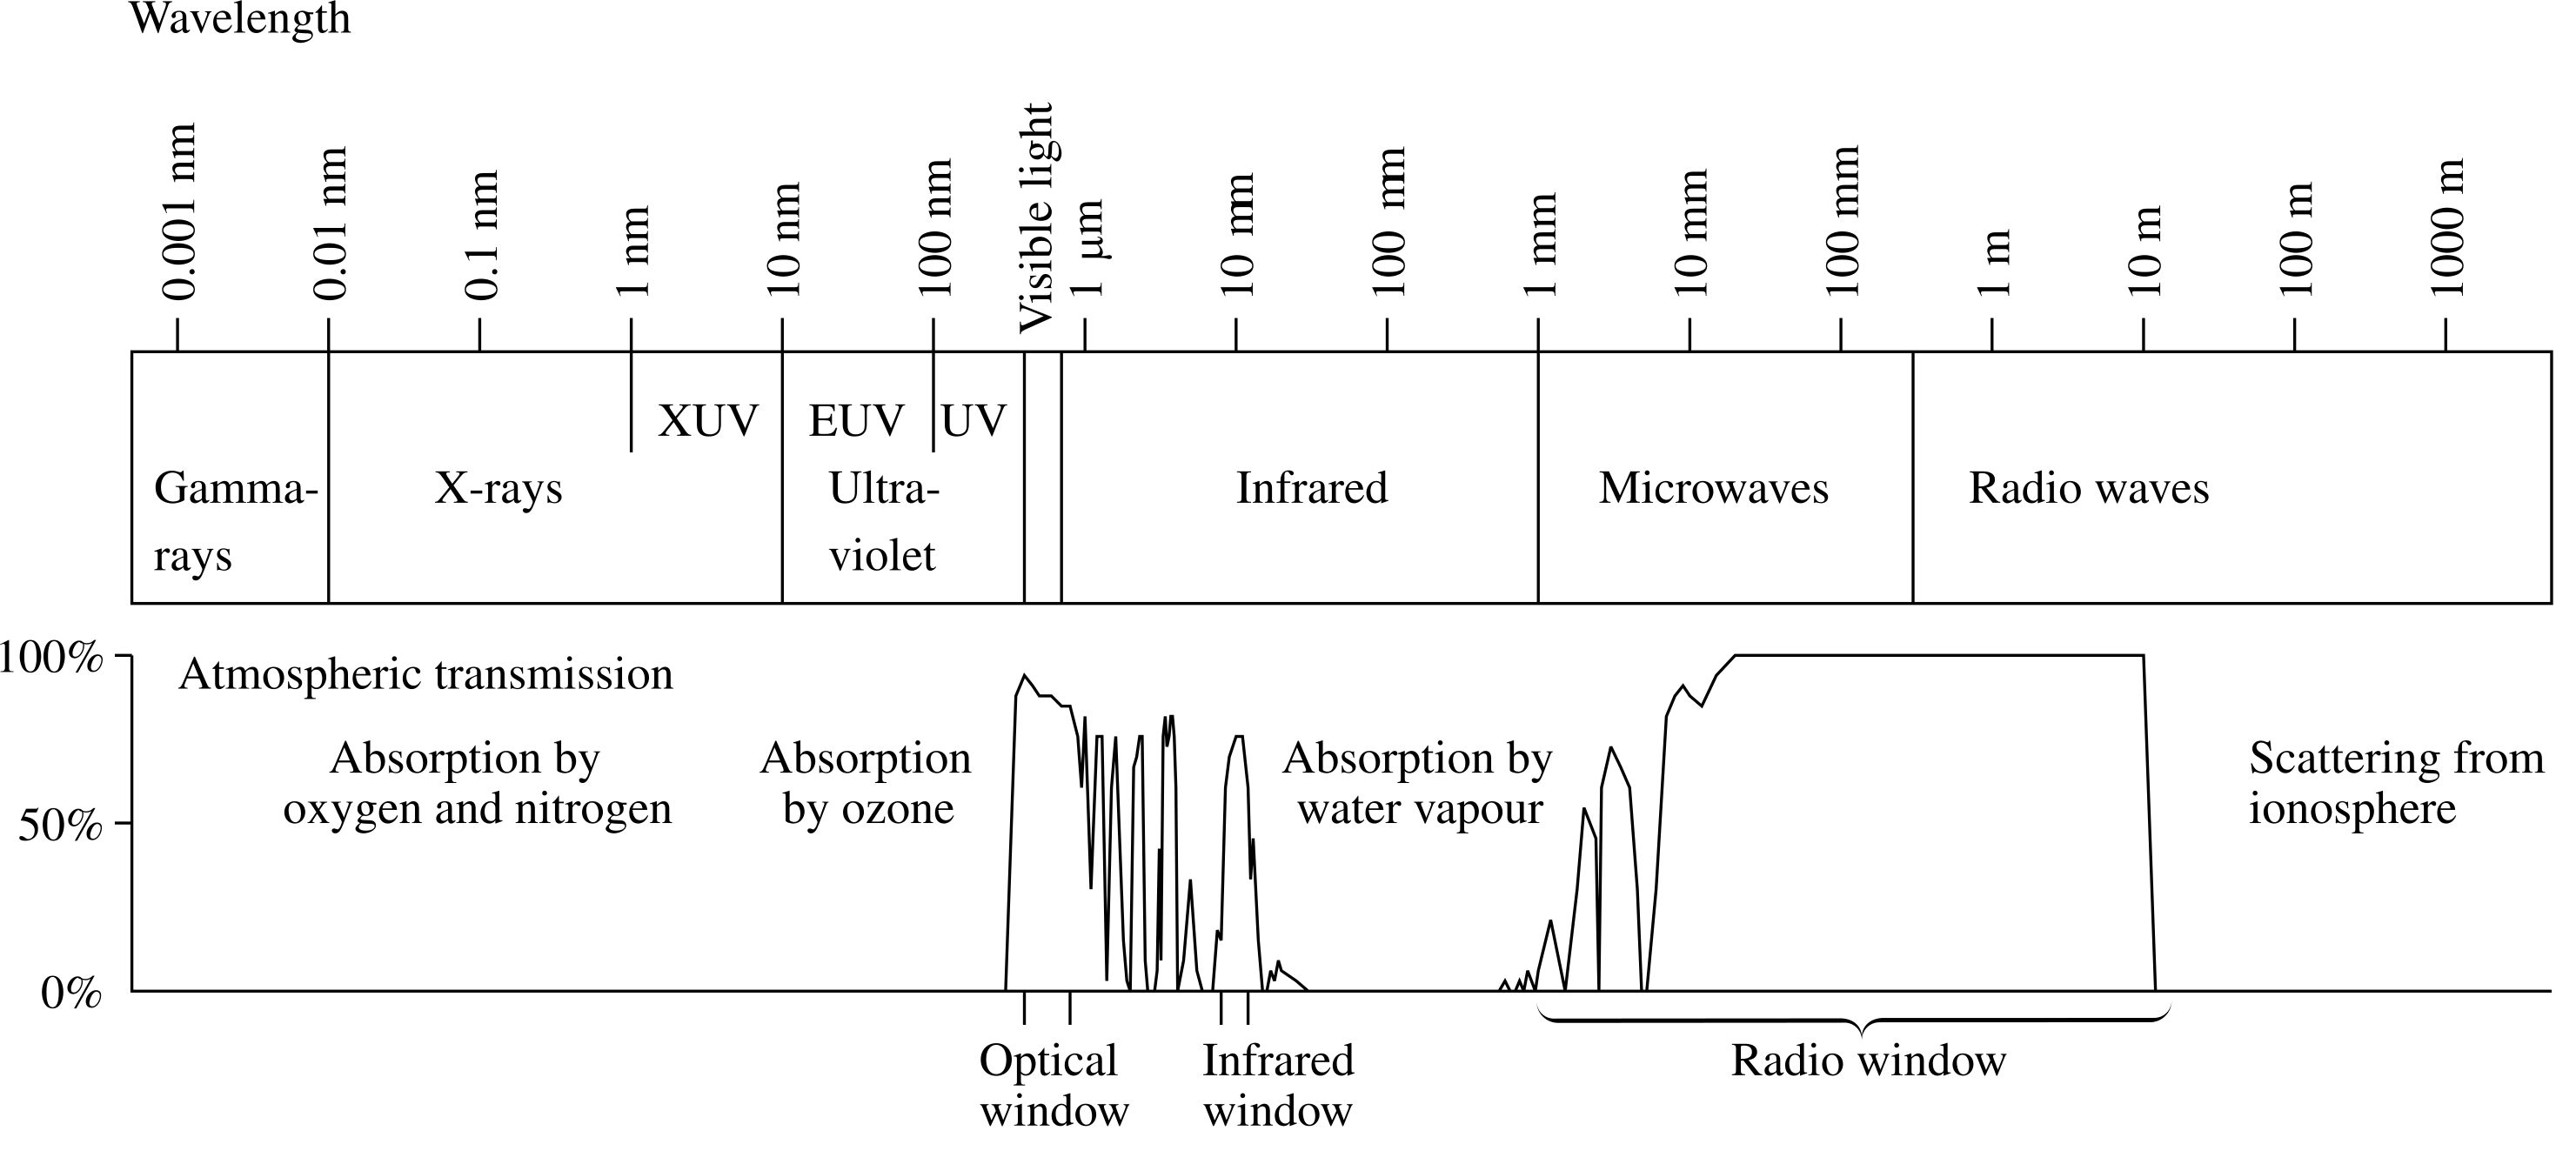
\includegraphics[width=\textwidth]{figures/atmosphere.png}
	\caption{Transmisión de la atmósfera a diferentes longitudes de onda. Figura tomada de \citet{karttunen2007fundamental}.}
	\label{fig:atmosphere-atenuation} 
\end{figure}

Por otro lado, que va desde los $ 300 \mathrm{nm} $ hasta los $ 800 \mathrm{nm} $, donde la atmósfera es casi transparente. A dicha región se le conoce como <<ventana óptica>> y gracias a ella es posible observar el cielo desde la superficie en ese rango de longitudes de onda. 

Algunas regiones de la luz infrarroja también puede observarse desde la superficie de la Tierra, como se ve en la Figura \ref{fig:atmosphere-atenuation}. Sin embargo, la mayor parte es absorbida por vapor de agua. La atmósfera también atenúa algunas regiones del microondas, pero es totalmente transparente a las ondas de radio. 

Todos los telescopios ópticos en la superficie funcionan gracias a la ventana óptica. Sin embargo, se han lanzado muchas misiones espaciales con telescopios que orbitan alrededor de la Tierra para tomar datos en el rango visible. Un ejemplo de ellos es el HST y recientemente el James Webb Space Telescope (JWST, \cite{gardner2023james}). El principio de recolección de luz de los telescopios es bastante simple: mientras más grande sea el espejo o el lente, más luz coleccionará. La cantidad de luz recibida por unidad de tiempo es directamente proporcional al área de recolección y ya que la mayoría de los espejos o lentes de los telescopios son circulares, esto significa que la proporción sigue la relación $ \pi r^2 $, donde $ r $ es el radio del espejo/lente. Debido a eso, los telescopios modernos son cada vez más grandes. Eso, junto con la optimización de los detectores han ayudado a que la astronomía crezca como ciencia. 


